\chapter{Results and Discussion}
iv.	Show feature correlation to diffuse, discuss cases based on images and corresponding irradiance components
In this chapter, we show results of applying the regression algorithms on our dataset for estimating DHI (Diffuse Horizontal Irradiance) from sky images. As the metric for comparison between methods, Root Mean Square Error(RMSE) is used. 

\section{Feature Selection}
Since the correlation of each feature element to DHI is not strong enough, we need to do a feature selection in order to select the most relevant features and discard the ones that are not helpful enough. For that purpose, we use a Forward-Selection algorithm for each method. This approach assumes an empty feature vector initially, and at every iteration evaluate the error of estimation after adding each one of the available feature elements to current feature set. The feature set with least error will be chosen and removed from available feature elements. However, the difference of last error and current error has to be more than a threshold for adding that feature elements. This helps to exclude random improvements caused by features and don't add them to final feature set. This threshold has been set empirically to 0.7 -60\% of inverse of chi-square cumulative distribution function of 1 degree of freedom- in RMSE.

%%%%%%%%%%%%%%%%%%%%%%%%%%%%%%%%%%%%%%%
\section{Linear Regression}

RMSE=60.7 on test and 64.4 on training
1 feature selected: clear-sky DHI

\begin{figure}[h]
\caption{Linear regression result using only non-image features}
\label{fig:ln_result_no_image}
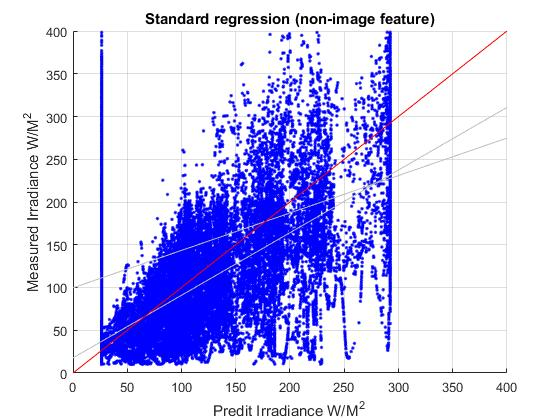
\includegraphics[scale=.5]{linear_regress_non_imag}
\centering
\end{figure}

RMSE=44.7 on test and 47.4 on training
12 feature selected out of 27.

\begin{figure}[h]
\caption{Linear regression result using all the features}
\label{fig:ln_result_all}
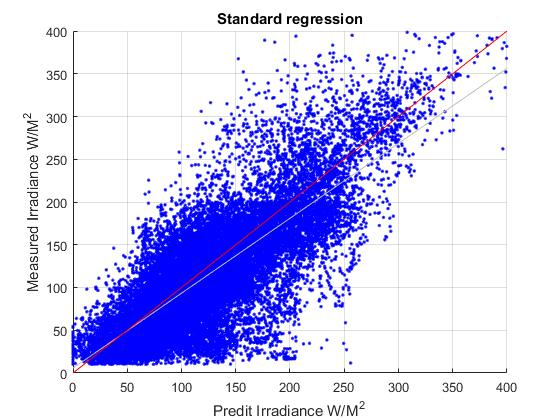
\includegraphics[scale=.5]{linear_regress_all}
\centering
\end{figure}

\begin{figure}[h]
\caption{Error histogram for linear regression}
\label{fig:ln_result_all}
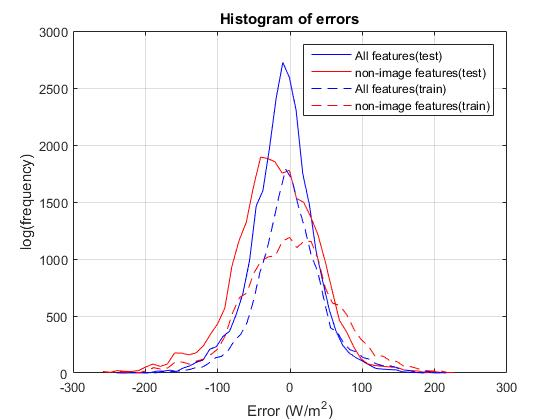
\includegraphics[scale=.5]{linear_regress_err_hist}
\centering
\end{figure}

%%%%%%%%%%%%%%%%%%%%%%%%%%%%%%%%%%%%%%%%%%
\section{K-NN}

RMSE=57.7 on test and 58.2 on training

\begin{figure}[h]
\caption{K-NN estimation result using only non-image features}
\label{fig:knn_result_no_image}
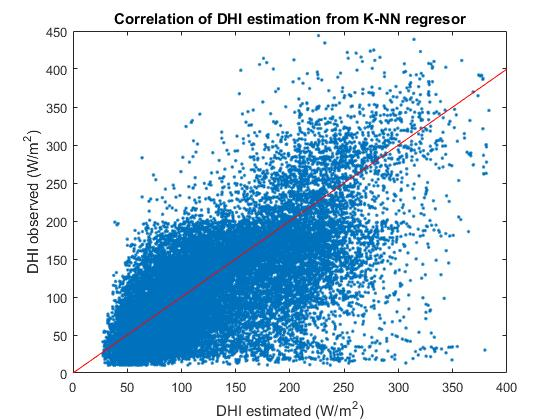
\includegraphics[scale=.5]{knn_result_no_image}
\centering
\end{figure}

RMSE=34.8 on test and 35.7 on training

\begin{figure}[h]
\caption{K-NN estimation result using all the features}
\label{fig:knn_result_all}
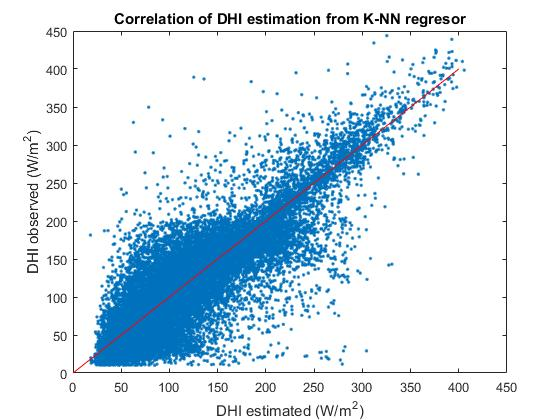
\includegraphics[scale=.5]{knn_result_with_image}
\centering
\end{figure}

\begin{figure}[h]
\caption{Error histogram for K-NN estimation result}
\label{fig:err_hist_knn}
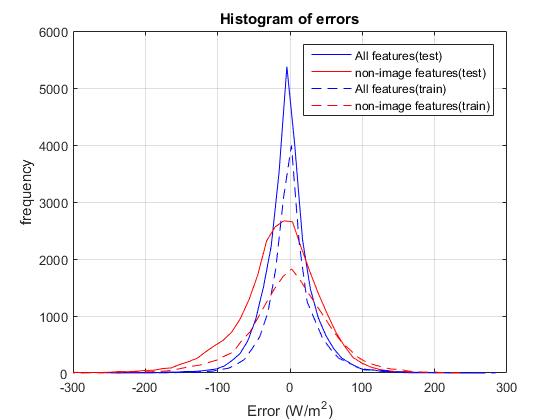
\includegraphics[scale=.5]{knn_result_error_hist}
\centering
\end{figure}

%%%%%%%%%%%%%%%%%%%%%%%%%%%%%%%%%%%%%%%
\section{SVR}
The performance of support vector regression is highly dependent on $C$, $\epsilon$ and $\gamma$ parameters which define trade off between model complexity (i.e. number of support vectors) and regression error and control influence of support vectors. Therefore, it is very important to tune these parameters on our specific dataset through k-fold cross validation. We are using 5-fold validation based on our training sample size. Thus, we randomly divide our training set into 5 equal sized partitions. Then for each parameter combination we use one of the folds for testing and the rest for training set. The final error of a parameter combination comes from averaging the errors for all the folds (5). After cross validation on $C$ and $\epsilon$  and $\gamma$ parameters

The result of SVR is depicted in Figure.

no-image : RMSE=68.2 on test and 67.2 on training

\begin{figure}[h]
\caption{SVR result using only non-image features}
\label{fig:svr_result_no_image}
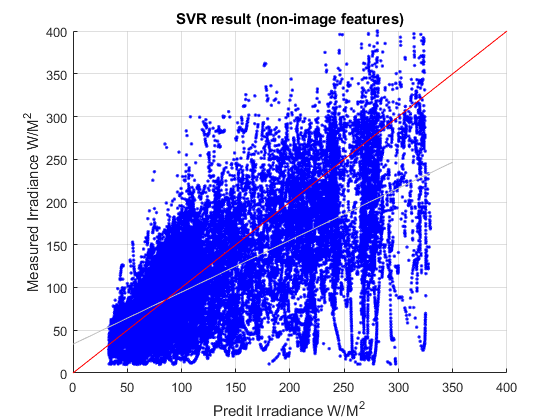
\includegraphics[scale=.5]{svr_result_no_image}
\centering
\end{figure}

RMSE=44.8 on test and 40.0 on training

\begin{figure}[h]
\caption{SVR result using all the features}
\label{fig:svr_result_all}
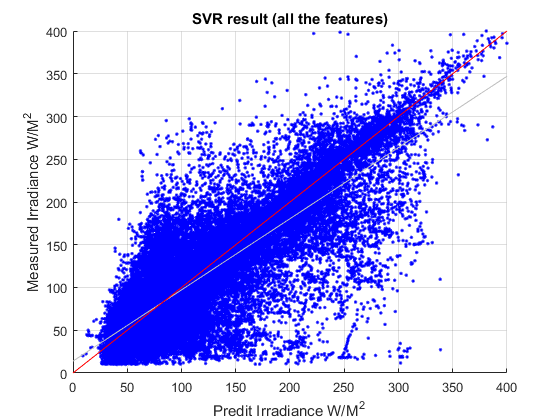
\includegraphics[scale=.5]{svr_result_all_features}
\centering
\end{figure}

\begin{figure}[h]
\caption{Error histogram for SVR result}
\label{fig:err_hist_svr}
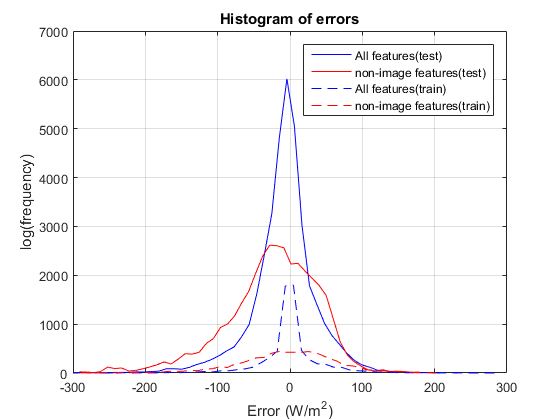
\includegraphics[scale=.5]{svr_error_histogram}
\centering
\end{figure}




